\documentclass[10pt,twocolumn]{article}
\usepackage[a4paper,margin=1.7cm,columnsep=0.7cm]{geometry}
\usepackage[T1]{fontenc}
\usepackage[utf8]{inputenc}
\usepackage{amsmath,amssymb}
\usepackage{graphicx}
\usepackage{booktabs}
\usepackage[section]{placeins}
\usepackage{array}
\newcolumntype{L}[1]{>{\raggedright\arraybackslash}p{#1}}
\usepackage{tikz}
\usetikzlibrary{arrows.meta,positioning,shapes.geometric,fit,calc}
\usepackage[hidelinks]{hyperref}
\usepackage[font=small,labelfont=bf,skip=3pt]{caption}
\usepackage{enumitem}
\setlist{nosep,leftmargin=1.3em}
\setlength{\parskip}{2pt}
\raggedbottom
\setlength{\tabcolsep}{3.2pt}
\setlength{\textfloatsep}{8pt plus 2pt minus 2pt}
\setlength{\floatsep}{6pt plus 2pt minus 2pt}
\setlength{\intextsep}{6pt plus 2pt minus 2pt}
\setlength{\dbltextfloatsep}{8pt plus 2pt minus 2pt}

\title{\textbf{ScholarLedger: Forgery-Resistant Academic Credentials on Ethereum with Private Commitments and Concurrent Batch Issuance}}
\author{Aryan Rastogi\\\small Roll no. 2310110439 \and Raghav Garg\\\small Roll no. 2310110697}
\date{\small CSD436 Blockchain Technology, course project\\[4pt] November 2026}

\begin{document}
\twocolumn[
\maketitle
\begin{abstract}
\noindent
ScholarLedger is a decentralized application (DApp) in which universities issue academic credentials on an Ethereum chain and anyone can verify them without a wallet. It addresses three weaknesses of hash-anchoring credential systems. First, the forgery attack of Zonneveld et al.\ on Block.co: a hash on a chain proves integrity but not who anchored it. ScholarLedger binds issuance to an on-chain registry of institutions, so the contract itself reverts a credential sent from an unregistered wallet. Second, privacy on a public chain: the chain stores only a salted SHA-256 commitment, and the student keeps a credential file that opens it. Third, volume on graduation day: an off-chain batch service, inspired by Block-STM and by optimistic concurrent execution of smart contracts, groups rows by conflicts, submits each conflict-free group without waiting and confirms it in one block, then anchors one Merkle root per batch. On a local Hardhat node, 50 conflict-free credentials took 310\,ms in one block against 2505\,ms over 50 blocks sequentially (about $8.1\times$; repeat runs gave $7.2$--$8.7\times$). The system has 24 contract tests and 13 service tests, all passing, and all six manual MetaMask checks passed with the real extension. An independent audit of the submission led to a final round of fixes, which we report with the limitations that remain. We state where the speedup comes from and what it does not show.
\end{abstract}
\vspace{10pt}
]

\section{Introduction}
\begin{figure*}[!t]
\centering
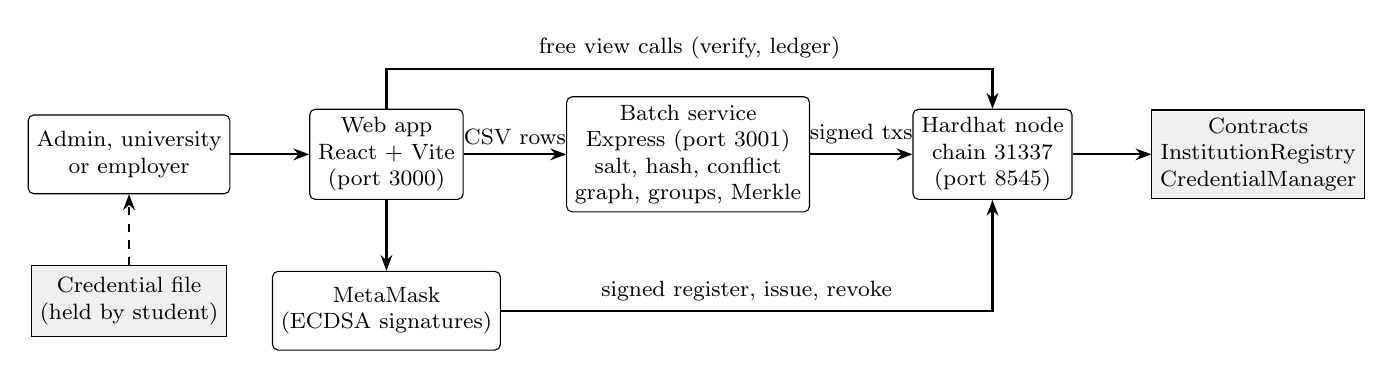
\begin{tikzpicture}[
  font=\footnotesize, node distance=6mm and 9mm,
  box/.style={draw, rounded corners=2pt, align=center, minimum height=10mm, inner sep=3pt, fill=white},
  store/.style={draw, align=center, minimum height=9mm, inner sep=3pt, fill=black!6},
  arr/.style={-{Stealth[length=2mm]}, thick}
]
\node[box] (u) {Admin, university\\or employer};
\node[box, right=10mm of u] (web) {Web app\\React + Vite\\(port 3000)};
\node[box, right=13mm of web] (svc) {Batch service\\Express (port 3001)\\salt, hash, conflict\\graph, groups, Merkle};
\node[box, right=13mm of svc] (node) {Hardhat node\\chain 31337\\(port 8545)};
\node[store, right=10mm of node] (con) {Contracts\\InstitutionRegistry\\CredentialManager};
\node[box, below=9mm of web] (mm) {MetaMask\\(ECDSA signatures)};
\node[store, below=9mm of u] (file) {Credential file\\(held by student)};
\draw[arr] (u)--(web);
\draw[arr] (web)-- node[above]{CSV rows} (svc);
\draw[arr] (svc)-- node[above]{signed txs} (node);
\draw[arr] (node)--(con);
\draw[arr] (web)--(mm);
\draw[arr] (mm.east) -| node[pos=0.25, above]{signed register, issue, revoke} (node.south);
\draw[arr] (web.north) -- ++(0,5mm) -| node[pos=0.25, above]{free view calls (verify, ledger)} (node.north);
\draw[arr, dashed] (file)--(u);
\end{tikzpicture}
\caption{ScholarLedger architecture. White boxes are programs; shaded boxes are contracts and the holder's file. Reads need no wallet; every write is a signed transaction.}
\label{fig:arch}
\end{figure*}
\textbf{Background.} A degree certificate is checked today by contacting the issuing university, which is slow, depends on the university's systems staying available, and trusts a database the university alone controls. Blockchain credential systems such as Block.co instead store a hash of the certificate on a public chain, so anyone can check that a document has not changed.

\textbf{Importance.} Zonneveld, Rafaiani and Baldi \cite{zonneveld2026} showed that this is not enough. Anyone with a wallet can anchor the hash of a forged degree, and the verifier then reports it as present on the chain. A hash proves \emph{integrity}; it does not prove \emph{authentication}, that a legitimate institution issued it. A second problem is privacy: anything written to a public chain is public forever, so student data cannot simply be stored there.

\textbf{Motivation.} Our midsem prototype bound issuance to registered institutions, but our midsem review found that the contract stored the student ID and program in clear text, and that the batch-issuing route was not wired to the right contract. The course also asked how transaction volume, threads and conflicts affect concurrent execution. A graduation day, when one university issues thousands of credentials at once, is a natural case for that question.

\textbf{Contributions.} We do not claim a new consensus protocol or a new cryptographic primitive. The contributions are a working system and its measurement:
\begin{itemize}
\item Identity-bound issuance: a registry contract plus a \texttt{require} on \texttt{msg.sender}, demonstrated against a side-by-side re-enactment of the Block.co attack, and a deregistration cutoff so that removing an institution does not void what it issued earlier.
\item Privacy by commitment: only a salted SHA-256 commitment on chain, a holder-kept credential file, and a verifier that detects an edited file before any chain call.
\item A concurrent batch engine with conflict graph, greedy grouping, validate-before-commit and one block per group, with a Merkle root, issuer and count recorded per batch.
\item A measured comparison of sequential and grouped issuance, with the source of the speedup stated plainly.
\item A web application in which every outcome (valid, revoked, issuer deregistered, not found, altered file, rejected forgery) is visible.
\end{itemize}

\section{Literature Review / Related Work}
\textbf{The forgery attack.} Zonneveld et al.\ \cite{zonneveld2026} analyse Block.co and show that a record can be tamper-evident without proving that its issuer is a real institution. Their key point, that integrity and issuer identity are separate properties, is the design rule of our registry. Our difference: we enforce the issuer check inside the contract, so a forged issuance never reaches the chain's state.

\textbf{Private certification.} Saramago, Meling and Jehl \cite{saramago2022} keep credentials off chain with the holder, publish commitments in an incremental Merkle tree, and use zero-knowledge proofs so that only the needed claims are revealed. We adopt the commitment and holder-kept file. We do not implement zero-knowledge proofs, so a credential file reveals all of its fields to whoever receives it.

\textbf{Block-STM.} Gelashvili et al.\ \cite{gelashvili2023} execute the transactions of a block speculatively in parallel, validate what each one read, and re-execute those that read stale data, keeping the result equal to sequential execution. We borrow the optimistic idea at the issuance level: conflict-free rows go out together, and a row that conflicts with an earlier one is validated before it is sent.

\textbf{Optimistic concurrent smart contracts.} Anjana et al.\ \cite{anjana2019} let miners run smart-contract transactions concurrently with BTO and MVTO software transactional memory and record conflicts in a block graph that validators replay in parallel. They report mean miner speedups of 3.6--3.7$\times$. Our midsem C++ benchmark followed this design (Section~\ref{sec:midsem}); the batch service reuses its conflict-graph idea.

\textbf{Evaluation practice.} Fern\'andez-Blanco et al.\ \cite{fernandez2024} build a forgery-prevention system and evaluate it on CPU-based and low-power computers. We follow their practice of reporting the machine, the parameters and concrete timings; we have not tested low-power hardware.

\section{Objective}
Build a working credential DApp that (1) accepts credentials only from registered institutions, (2) stores no student data on the public chain, (3) lets anyone verify a credential for free and without a wallet, (4) lets only the original issuer revoke, and (5) issues large batches concurrently with conflict detection and one Merkle root per batch. Then measure what the batch engine gains over sequential issuance, and test every outcome end to end.

\section{Proposed System}
Figure~\ref{fig:arch} shows the architecture. Three programs run locally. A Hardhat node (chain ID 31337) holds two Solidity contracts. A React web app reads the chain directly for verification and asks MetaMask to sign registration, issuance and revocation. A Node.js batch service signs batch transactions with the demo university's key on the server, so no private key is ever sent from the browser. Because that service can sign as a university, it listens on the loopback interface only, accepts requests only from the web app's origin, and can require a bearer token.



\textbf{Contracts.} \texttt{InstitutionRegistry} maps an address to a name, domain, registration time, active flag and a validity cutoff; only the deployer (the admin) can register or deregister, and a deregistered address can never be registered again. \texttt{CredentialManager} stores, per commitment, the issuer, the issue time and a revoked flag, and per batch a Merkle root, issuer, count and time. Table~\ref{tab:functions} lists the functions. No string about a student appears in storage or in any event.

\begin{table}[!t]
\caption{Contract functions, who may call them, and their checks.}
\label{tab:functions}
\centering\footnotesize
\begin{tabular}{@{}L{2.85cm}L{1.3cm}L{3.75cm}@{}}
\toprule
function & caller & checks and effect\\
\midrule
\texttt{registerInstitution} & admin & non-zero address never registered before, name and domain not empty\\
\texttt{revokeInstitution} & admin & must be active; sets a cutoff $\le$ now; credentials issued before it stay valid\\
\texttt{issueCredential} & registered & sender registered, commitment non-zero and new; stores issuer, time\\
\texttt{verifyCredential} & anyone (view) & valid = exists, not revoked, issued while the issuer was authorized\\
\texttt{revokeCredential} & original issuer & still registered; exists, not yet revoked\\
\texttt{storeMerkleRoot} & registered & root non-zero, $1\le$ count $<2^{32}$; returns a batch id\\
\bottomrule
\end{tabular}
\end{table}

\textbf{Web app.} Eight pages: Home (live statistics and explanation), Verify, Issue, Batch issue, Revoke, Register, Ledger and Forgery demo. Verification uses a read-only provider, so an employer needs no wallet.

\section{Methodology}

\subsection{Identity-bound issuance}
\texttt{issueCredential} begins with
\[
\texttt{require(registry.isRegistered(msg.sender))}.
\]
Inside the EVM, \texttt{msg.sender} is recovered from the transaction's ECDSA signature, so a wallet cannot claim another's address. A forger's wallet is not in the registry, the call reverts with ``Issuer not registered'', and nothing is stored. Revocation checks that the caller is the stored issuer and is still registered. Deregistration takes a cutoff time: a university that closes passes the current time, and one whose key leaked passes the time of the leak. A credential is valid only if it was issued before its issuer's cutoff, so removing an institution neither voids its earlier graduates nor, because an address can never be re-registered, revives anything.

\subsection{Commitments and the credential file}
For each credential the issuer draws a 32-byte random salt $s$ and computes
\begin{equation}
c = \mathrm{SHA256}(s \,\|\, \texttt{|} \,\|\, \mathit{id} \,\|\, \texttt{|} \,\|\, \mathit{prog} \,\|\, \texttt{|} \,\|\, \mathit{meta}),
\end{equation}
where $\|$ is string concatenation and fields are trimmed. The pipe separates the fields, so it is forbidden inside them: the batch service, the Issue form and the verifier all reject a \texttt{|} in any field, which makes the split, and therefore the commitment, unambiguous. Only $c$ goes on chain. The student receives a JSON file holding $s$, the fields, $c$, the issuer, the chain and contract, and, for batch credentials, a Merkle proof. The browser (WebCrypto) and the batch service (Node \texttt{crypto}) must agree; both test one fixed vector (64 zero characters, \texttt{S1}, \texttt{BTech}, empty metadata).

To verify a file, the page recomputes $c$ from the file. If it differs from the file's own commitment, the page reports ``Altered file'' and makes no chain call. Otherwise it calls \texttt{verifyCredential(c)} and shows one of five outcomes: valid, revoked, issuer deregistered, not found, or altered. Without the salt nobody can test guesses of student IDs against the public commitments.

\subsection{Merkle root per batch}
The batch service builds a SHA-256 Merkle tree over the successful commitments of a batch. A parent is
\begin{equation}
h_{\text{parent}} = \mathrm{SHA256}(h_{\text{left}} \,\|\, h_{\text{right}}),
\end{equation}
over lowercase hex strings, and any level with an odd count duplicates its last node. The root, issuer and count are stored with \texttt{storeMerkleRoot}; each credential file carries the sibling hashes from its leaf to the root. The verifier recomputes the root and also checks that the stored batch was issued by the same institution as the credential.

\subsection{Optimistic concurrent batch issuance}
Two rows $r_i, r_j$ conflict when they name the same student and program:
\begin{equation}
r_i \sim r_j \iff \mathit{id}_i = \mathit{id}_j \wedge \mathit{prog}_i = \mathit{prog}_j .
\end{equation}
The commitment cannot be the conflict key, because random salts make every commitment unique. The engine builds the conflict graph with a hash map from key to rows, then colours it greedily: each row joins the first group containing no row it conflicts with, so a repeated row lands in a later group. Groups run in order; the rows of a group run concurrently with \texttt{Promise.all}.

\textbf{Validate before commit.} Before a row of a later group is sent, the service checks whether its key was already issued earlier in the same request; if so it aborts without sending (``Duplicate of an earlier row in this batch''). This is the optimistic validation step of OCC: optimistic grouping, validation, then commit or abort.

\textbf{Nonces and one block per group.} An Ethereum account's transactions must carry consecutive nonces. The service reads the pending nonce once and hands out nonces itself, takes each nonce synchronously before any \texttt{await}, fetches fee data once, and sets a fixed gas limit (200{,}000; an issue uses about 59{,}000) so a reverted transaction still consumes its nonce and leaves no gap. On the local chain it turns Hardhat's automine off, submits every row of the group, mines one block, waits for all receipts, and turns automine back on in a \texttt{finally} block. Each row and the root transaction wait at most 30\,s for a receipt. A credential file is built as soon as its row confirms and all files are written to disk before the root is anchored, so a failure in the root step returns the files with an error instead of losing them (checked by deregistering the issuer in the middle of a 40-row batch: 15 rows confirmed and all 15 files came back). A request may hold at most 1{,}000 rows.

\textbf{What this is and is not.} The EVM still executes the transactions of a block one after another. The gain comes from pipelining: a group's rows are submitted without waiting for each other and confirmed in one block, instead of one round trip and one block per row. True parallel execution inside the node is what Block-STM and Anjana et al.\ do; our midsem benchmark simulated that part.

\subsection{Midsem study: proof of work and concurrent execution}
\label{sec:midsem}
For the midsem assignment we generated 400 simulated transactions (100 for each of four contract functions, seeded with the roll number), built a genesis block and three data blocks of at most 150 transactions, and mined each with SHA-256 until the hash started with \texttt{39} (mean 166.7 attempts per block). A C++17 benchmark then ran the same transactions serially and with a BTO-style concurrent miner and a graph-following validator, following Anjana et al. Section~\ref{sec:results-midsem} summarises its results.

\section{Experimentation and Results}

\subsection{Setup}
One laptop: Intel Core i5-11400H (6 cores, 12 threads), about 8\,GB RAM, Windows 11. Hardhat 2 local node (chain 31337), Solidity 0.8.20, ethers.js 6, Node.js. Times come from the batch service's own metrics (milliseconds from batch start); a ``block'' is a Hardhat block. Nothing was tuned on the measured runs.

\subsection{Batch throughput}
Table~\ref{tab:batch} compares the two modes on 50 conflict-free rows. Sequential mode sends one row and waits for its receipt before the next; grouped mode is the engine of Section 5.4. The Batch page's ``Compare with sequential'' runs both on the same rows and draws them on one time axis (Figure~\ref{fig:compare}).

\begin{table}[!t]
\caption{50 conflict-free rows, local Hardhat node. Speedup is sequential time over grouped time of the same run pair.}
\label{tab:batch}
\centering\footnotesize
\begin{tabular}{@{}lrrrr@{}}
\toprule
run & time (ms) & tx/s & blocks & speedup\\
\midrule
A, sequential & 2505 & 20.0 & 50 & \\
A, grouped & 310 & 161.3 & 1 & $8.1\times$\\
B, sequential & 2595 & 19.3 & 50 & \\
B, grouped & 358 & 139.7 & 1 & $7.2\times$\\
\bottomrule
\end{tabular}
\end{table}

\begin{figure}[!t]
\centering
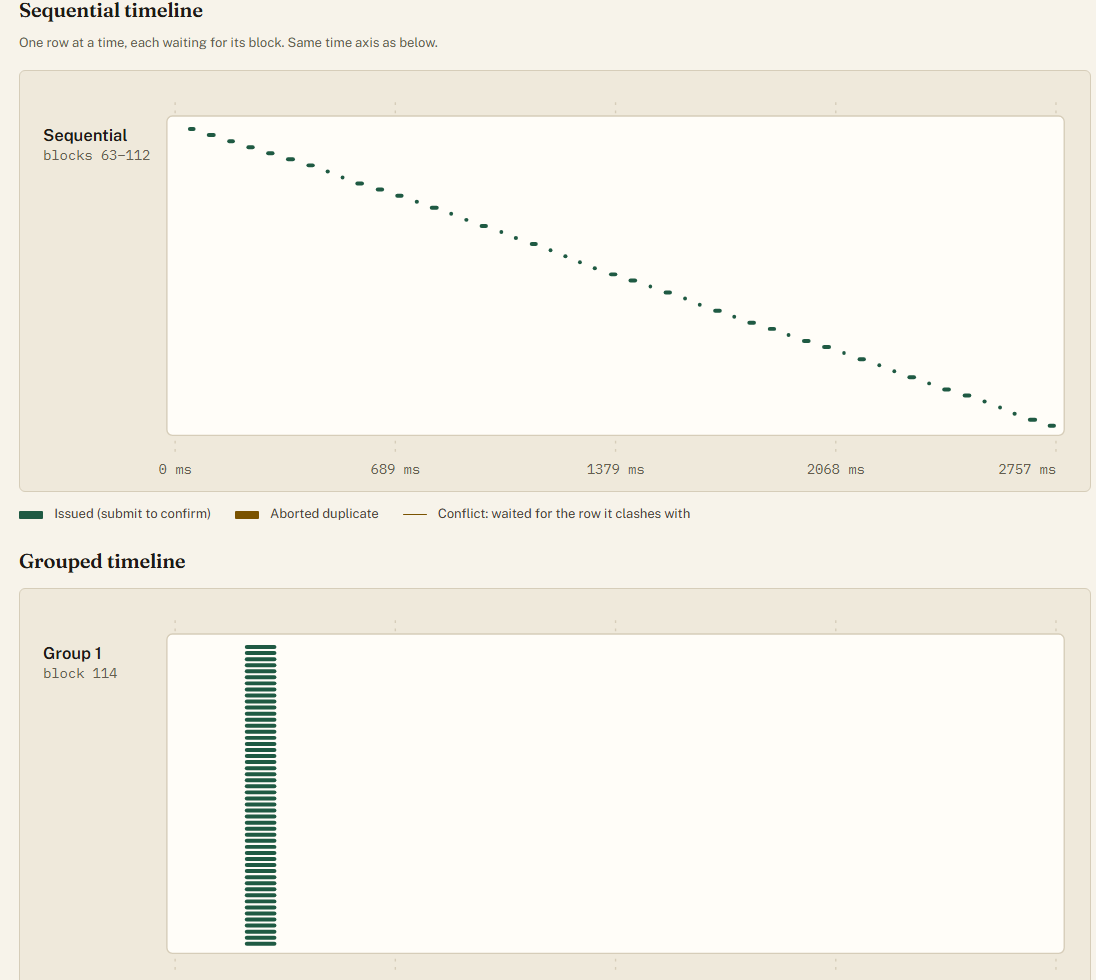
\includegraphics[width=\columnwidth]{figures/compare.png}
\caption{The two timelines of one comparison run (50 rows, same time axis). Each bar runs from submit to confirm. Sequential rows form a staircase over 50 blocks; grouped rows form one column in a single block.}
\label{fig:compare}
\end{figure}

\textbf{What these show.} Grouping saves about $7$--$8\times$ on this machine (a third comparison run in the web app gave $8.7\times$). In a 30-row batch with 3 repeated students, the 27 valid rows were confirmed in one block and the 3 repeats were aborted before sending, in 279\,ms. The figures come from single runs on one machine and vary between runs. On a public chain the network decides block packing, so the shape, not these numbers, carries over.

\subsection{Gas}
Table~\ref{tab:gas} gives gas used from transaction receipts. Replacing an array of every commitment, kept only for its length, by a counter removed one storage write per issue (about 22{,}000 gas); making the registry reference \texttt{immutable} saved about 2{,}100 more. Deregistration support made \texttt{registerInstitution} and \texttt{revokeCredential} slightly more expensive.

\begin{table}[!t]
\caption{Gas used, from receipts on the local node.}
\label{tab:gas}
\centering\footnotesize
\begin{tabular}{@{}lr@{}}
\toprule
transaction & gas\\
\midrule
\texttt{issueCredential} (array, first version) & 82{,}857\\
\texttt{issueCredential} (final) & 58{,}680\\
\texttt{issueCredential}, first on a fresh contract & 75{,}780\\
\texttt{storeMerkleRoot} (3 rows) & 98{,}515\\
\texttt{registerInstitution} & 164{,}339\\
\texttt{revokeInstitution} (deregister) & 31{,}913\\
\texttt{revokeCredential} & 35{,}543\\
\bottomrule
\end{tabular}
\end{table}

\subsection{Correctness and end-to-end checks}
Automated tests: 24 contract tests (Mocha and Chai, run by \texttt{npm test}) cover access control, the forgery rejection, duplicate rejection, revocation rules, input validation, the deregistration cutoff, the batch limits, that \texttt{CredentialIssued} has three inputs and none is a string, and the commitment test vector. Thirteen batch-service tests (\texttt{node:test}) cover grouping of duplicates, Merkle proofs for every leaf of trees with 1, 2, 3, 5, 6 and 7 leaves, root change on a changed leaf, timing fields, an unknown mode, the pipe character, the row limit, the token check and a foreign browser origin. All pass.

Table~\ref{tab:manual} lists the manual checks run with the real MetaMask extension against a fresh deployment, every transaction on chain 31337. They were run before the final audit fixes; the changed contract rules are covered by the automated tests.

\begin{table}[!t]
\caption{Manual checks with MetaMask (account \#0 admin, \#1 Demo University, \#2 unregistered). All passed.}
\label{tab:manual}
\centering\footnotesize
\begin{tabular}{@{}L{3.3cm}L{0.8cm}L{3.75cm}@{}}
\toprule
check & acct. & observed\\
\midrule
Forgery demo & \#2 & simulated side ``accepted''; contract ``not a registered institution''\\
Register \#2 as institution & \#0 & confirmed in block 5\\
Issue S9/BTech, verify file & \#1 & confirmed in block 4; file Valid\\
Revoke S9 from wrong account & \#2 & ``only the institution that issued \ldots''\\
Revoke as issuer, verify & \#1 & confirmed in block 6; file Revoked\\
Wallet on another network & -- & warning chip ``expected 31337''\\
\bottomrule
\end{tabular}
\end{table}

\begin{figure}[!t]
\centering
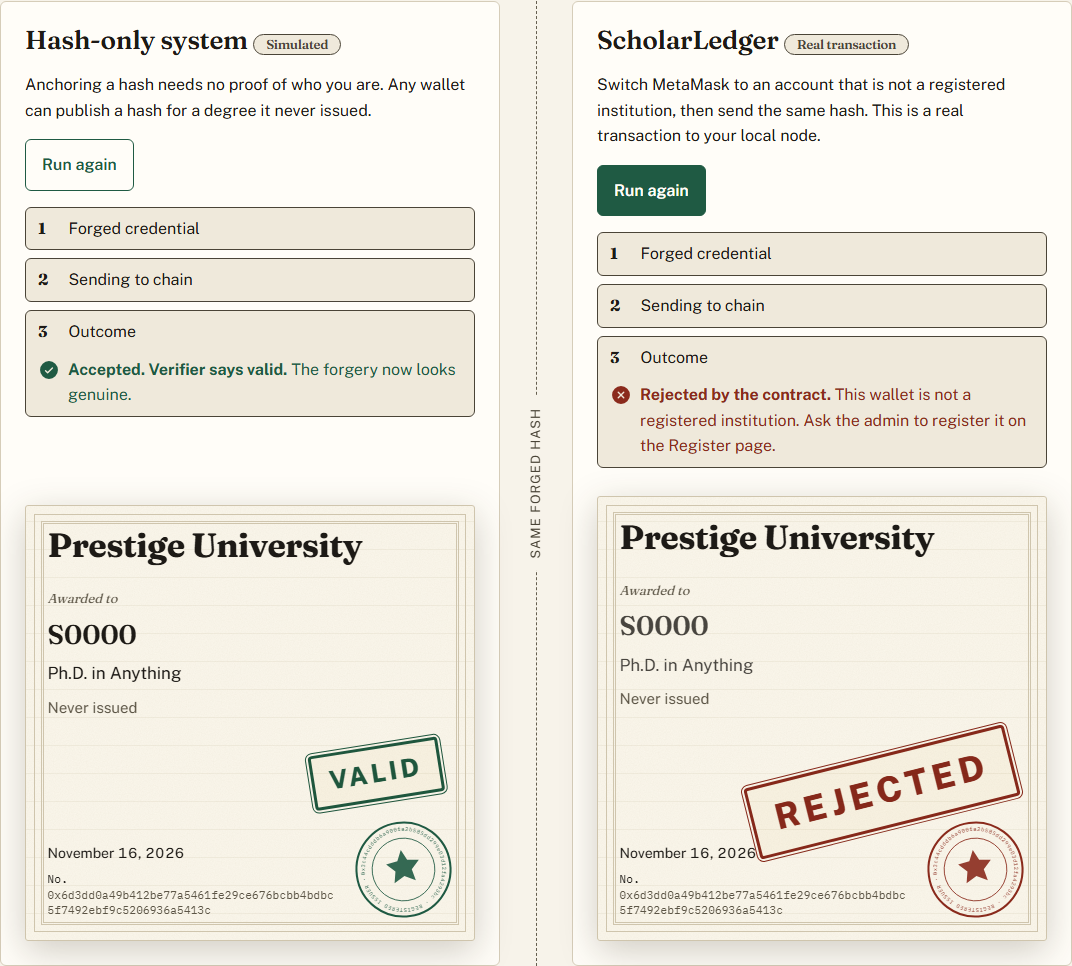
\includegraphics[width=\columnwidth]{figures/forgery.png}
\caption{Forgery demo with the same forged hash. Left: a simulated hash-only system accepts it. Right: the same call from an unregistered wallet; the wallet simulates it first, the contract refuses it, and nothing is broadcast.}
\label{fig:forgery}
\end{figure}

\begin{figure}[!t]
\centering
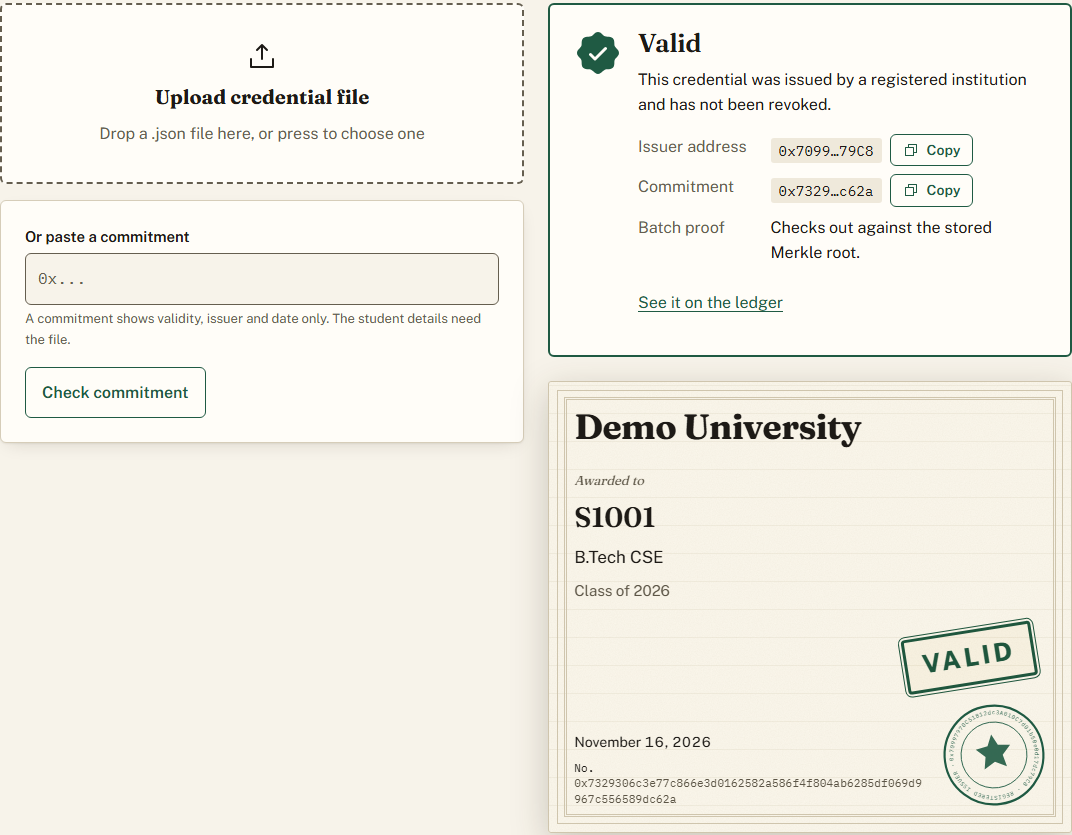
\includegraphics[width=\columnwidth]{figures/verify.png}
\caption{Verify page after uploading a batch credential file: status, issuer, commitment, batch-proof check and the credential drawn as a certificate.}
\label{fig:verify}
\end{figure}

\subsection{Midsem concurrency benchmark}
\label{sec:results-midsem}
Tables~\ref{tab:threads} and \ref{tab:conflict} summarise the C++ benchmark (30 measured runs after 3 warm-ups; medians). Varying the batch from 50 to 500 transactions at 25\% conflict with 8 or 16 workers gave miner speedups of $2.6$--$4.0\times$ and validator speedups of $2.7$--$4.3\times$, growing with batch size. With one worker the STM machinery is slower than serial; from four workers on both miner and validator gain, best at 16 workers (oversubscribed on 12 hardware threads). Raising the share of conflicting transactions from 10\% to 90\% multiplied the conflict-graph edges from 30 to 270 but left the longest dependency path at 4--5 and the speedup near $3.8$--$3.9\times$: duplicates fail their checks and verification mostly reads, so more conflicts did not create long chains of dependent writes.

\begin{table}[!t]
\caption{Midsem C++ benchmark, varying workers (100 transactions, 25\% conflict). Speedup is serial median over concurrent median.}
\label{tab:threads}
\centering\footnotesize
\begin{tabular}{@{}lrrrrr@{}}
\toprule
workers & 1 & 2 & 4 & 8 & 16\\
\midrule
miner speedup & 0.91 & 1.05 & 1.77 & 2.88 & 3.21\\
validator speedup & 0.95 & 0.99 & 1.81 & 3.17 & 3.26\\
\bottomrule
\end{tabular}
\end{table}

\begin{table}[!t]
\caption{Midsem C++ benchmark, varying conflict (300 transactions, 16 workers; medians).}
\label{tab:conflict}
\centering\footnotesize
\begin{tabular}{@{}lrrrrr@{}}
\toprule
conflict & edges & path & miner & validator & failures\\
\midrule
10\% & 30 & 4 & $3.76\times$ & $4.16\times$ & 20\\
25\% & 74 & 5 & $3.78\times$ & $4.17\times$ & 53\\
50\% & 150 & 4 & $3.82\times$ & $3.95\times$ & 110\\
90\% & 270 & 4 & $3.92\times$ & $4.03\times$ & 200\\
\bottomrule
\end{tabular}
\end{table}

\subsection{Security analysis}
Table~\ref{tab:security} checks the security properties against the code.

\begin{table}[!t]
\caption{Threats on a public chain and what the system does.}
\label{tab:security}
\centering\footnotesize
\begin{tabular}{@{}L{2.4cm}L{4.0cm}L{1.5cm}@{}}
\toprule
threat & mitigation & status\\
\midrule
Forged issuance & registry check on \texttt{msg.sender} & done\\
Open batch endpoint signing as a university & loopback bind, origin allow-list, optional token & done (local)\\
Files lost if a batch fails late & files saved before anchoring and always returned & done\\
Deregistration voiding old credentials & validity cutoff; no re-registration & done\\
Student data exposure & salted commitment only; file with holder & done\\
Edited credential file & commitment recomputed before any chain call & done\\
Unauthorized revocation & only the stored issuer & done\\
Duplicate commitment & rejected by the contract & done\\
Duplicate student across batches & not detectable on chain & limitation\\
Admin key compromise & single admin key, no multisig & limitation\\
Another institution squatting a commitment & credentials keyed by commitment only & limitation\\
Private key in browser & batch key held server-side & done (local)\\
\bottomrule
\end{tabular}
\end{table}

\section{Conclusions and Limitations}
ScholarLedger shows that a credential DApp can close the Block.co forgery attack at the contract level, keep every student detail off a public chain, and issue large batches several times faster by grouping conflict-free rows and confirming each group in one block. The forgery is rejected by the network itself, verification is free and needs no wallet, and every outcome is visible in the web app and covered by automated or manual tests.

\textbf{Limitations.} (1) The speedup is measured on a local Hardhat node where we control block production; it comes from pipelining submissions, not from parallel execution inside the EVM, and the numbers are from single runs on one laptop. (2) The admin is one key, and vetting institutions remains a trust decision. (3) The contract cannot detect the same student issued twice with different salts; the service only dedupes within a batch. (4) A credential file reveals all of its fields; there is no selective disclosure. (5) The batch service signs with a key held by the server; binding it to the loopback interface makes it acceptable for a local demonstration only, and institution-signed batches are the real fix. (6) Credentials are keyed by commitment alone, so a registered institution that front-runs another's commitment becomes its recorded issuer. (7) The Merkle tree duplicates the last node of odd levels and does not separate leaf and node hashes; the verifier also requires the leaf to exist as a credential. (8) We have not deployed to a public testnet or measured low-power hardware, and the local chain is in memory, so it is wiped on restart.

\textbf{Future work.} Deploy to the Sepolia testnet and measure real gas and latency; replace the admin with a multisig or a consortium of accreditation bodies; add zero-knowledge selective disclosure following Saramago et al.; detect cross-batch duplicates with an issuer-keyed tag; let institutions sign batches with their own wallets (an EIP-712 signature over the Merkle root, checked with \texttt{ecrecover}); key credentials by issuer and commitment; and compare with Block-STM-style parallel execution inside the node.

\begin{thebibliography}{99}\footnotesize
\bibitem{zonneveld2026} Zonneveld, G., Rafaiani, G. and Baldi, M., 2026. A forgery attack on the Block.co blockchain-based digital credential certification system. \textit{arXiv:2606.31462}.
\bibitem{saramago2022} Saramago, R. Q., Meling, H. and Jehl, L. N., 2023. A privacy-preserving and transparent certification system for digital credentials. In \textit{26th International Conference on Principles of Distributed Systems (OPODIS 2022)}, LIPIcs 253 (pp. 9:1--9:24).
\bibitem{gelashvili2023} Gelashvili, R., Spiegelman, A., Xiang, Z., Danezis, G., Li, Z., Malkhi, D., Xia, Y. and Zhou, R., 2023. Block-STM: Scaling blockchain execution by turning ordering curse to a performance blessing. In \textit{Proceedings of the 28th ACM SIGPLAN Symposium on Principles and Practice of Parallel Programming} (pp. 232--244).
\bibitem{anjana2019} Anjana, P. S., Kumari, S., Peri, S., Rathor, S. and Somani, A., 2019, February. An efficient framework for optimistic concurrent execution of smart contracts. In \textit{27th Euromicro International Conference on Parallel, Distributed and Network-Based Processing (PDP)}. doi:10.1109/PDP.2019.00020.
\bibitem{fernandez2024} Fern\'andez-Blanco, G., Froiz-M\'iguez, I., Fraga-Lamas, P. and Fern\'andez-Caram\'es, T. M., 2024. A blockchain based system for preventing academic forgery: Design and practical evaluation for CPU-based and low-power computers. In \textit{2024 6th International Conference on Blockchain Computing and Applications (BCCA)} (pp. 406--413). IEEE.
\bibitem{solidity} Solidity documentation, ``Security considerations''. \url{https://docs.soliditylang.org}.
\end{thebibliography}

\end{document}
